\documentclass[main.tex]{subfiles}\begin{document}


\chapter{Concept} \label{chap:Concept}


\begin{figure}[H]
    \centering
    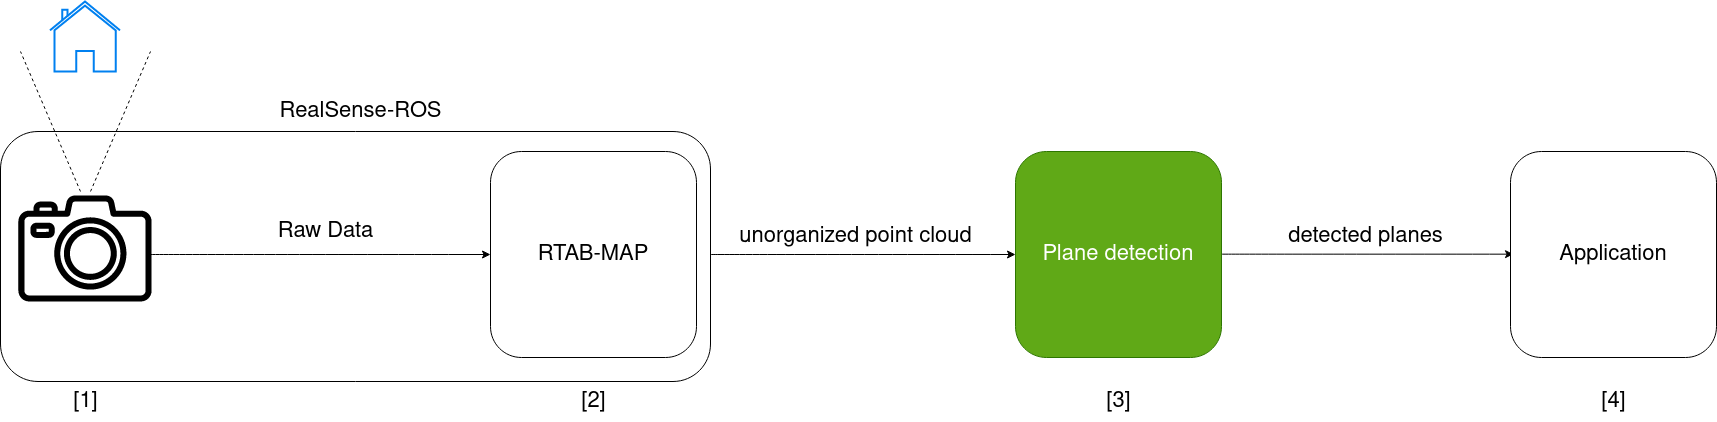
\includegraphics[width=15 cm]{images/concept_specific.png}
    \caption[AR/VR System Overview]{The procedure of the plane detection process. The specialized sensor records data ([1]), which is passed to
        a SLAM algorithm ([2]). After map assembly, a point cloud is handed to a plane detection algorithm ([3]).
        The detected planes are given to a use-case-specific application ([4]).}
    \label{fig:concept}
\end{figure}

Many AR and VR Systems integrate plane detection into their software. Some use it only to calculate the ground floor while others use plane detection to build a smaller model of the environment.
Figure~\ref{fig:concept} shows a generic block diagram of such a VR/AR system including plane detection.
The environment is continuously recorded by a specialized sensor, which is usually a camera, a depth sensor, or a combination thereof ([1]). A SLAM algorithm then integrates the new data into its already existing map ([2]). The map, in form of a point cloud, is subsequently passed to a plane detection algorithm ([3]). The algorithm performs the necessary steps to detect all planes inside the current map and passes the planes to the application ([4]).
The application then further processes those planes as required by the underlying use case.

To remove any noticeable delay in the application, the plane detection step has to run within a specific time limit. This temporal constraint is henceforth referred to as \textit{real-time}.
We introduce a precise definition of \textit{real-time} in Section~\ref{sec:realtime}.

When creating such an AR/VR system, the choice of plane detection algorithm is naturally of great importance. The problem is that most published algorithms are inherently incomparable.
Often different datasets or metrics are used, which precludes a quantitative comparison.
Moreover, algorithms are often incomparable by internal functionality due to differences in inputs and the format of the detected planes. Plane detection algorithms are, in some cases, developed to run on specific hardware.
We can safely conclude that selecting a single 'best' algorithm, solely based on the results presented in their respective work, is impossible.

To determine the \textit{real-time} applicability in a realistic environment, we perform a uniform comparison of plane detection algorithms. Therein, we especially pay attention to the accuracy and the calculation times of an algorithm. 
This comparison will thereby yield the algorithm that produces the best results as well. 
However, to perform this evaluation, we need the following:

\begin{enumerate}
    \item \label{enum:pda}Appropriate plane detection algorithms,
    \item \label{enum:ds} a useful dataset, \textit{and}
    \item \label{enum:rt} a definition of \textit{real-time}.
\end{enumerate}
The following sections are dedicated to these requirements.

\section{Selection of Plane Detection Algorithms}\label{sec:pdaselection}

Since most algorithms differ in certain aspects, it is not possible to compare them all uniformly.
Furthermore, not all algorithms are created out of the same motivation and, therefore, focus on different things.
Evaluating an algorithm in a scenario it has not been designed for is likely to yield meaningless results.
It is, therefore, necessary to first define objective criteria to superficially determine which algorithm shows relevance for the context of this work.


\subsection{Criteria}
\label{subsec:criteria}
In the following paragraphs, we outline appropriate criteria for the objective assessment of plane detection algorithms.

\paragraph{Type of Input}\label{par:input}
The first criterion is the type of input expected by a plane detection algorithm.
Allowing vastly different inputs is likely to render the evaluation more complicated, if not impossible, because an equivalent transformation
between two input types is not always possible.

We detail the different types of input in Section~\ref{sec:dataformats}. To reiterate, the data representation of the recorded
environment falls into one of four categories:
\begin{itemize}
    \item \textit{unorganized} or \textit{unstructured point cloud} (UPC),
    \item \textit{organized} or \textit{structured point cloud} (OPC),
    \item Depth-Image (DI), \textit{and}
    \item RGB-Image (RGBI),
\end{itemize}
whereas OPC and UPC both describe point clouds in the cartesian coordinate system. The primary difference is that the 3D coordinates inside
an \textit{organized} point cloud are saved in a 2D grid, while the \textit{unorganized} point cloud resembles an unsorted 1D array. Moreover, the 
Like OPC, depth images are a 2D grid of values. However, in contrast to the 3D coordinates of an OPC, the data points of depth images
are the distances to the sensor.



\paragraph{Detected Plane Format} \label{subsec:planeformat}
Which specific representation the detected planes take the form of is also essential.
If no uniform output type can be determined, consequently, no uniform metric for comparison can also be found.

In this work, we differentiate between the following:
\begin{itemize}
    \item 3D-inliers (3D-IN),
    \item 2D-inliers (2D-IN), \textit{and}
    \item the plane's normal vector and distance to origin ($n,d$),
\end{itemize}
whereas the \textit{3D-inliers} of a plane are a set of 3D points in the format of an $UPC$.
In contrast, \textit{2D-inliers} are two-dimensional representations of a plane.
This includes all methods to describe a plane in a two-dimensional manner, e.g., sets of indices, pixels or segmentation masks. These \textit{plane formats} generally correspond to two-dimensional input formats like \textit{organized point clouds} or \textit{(depth-) images}.

Lastly, planes are often described mathematically over their normal vector $n$ and distance to the origin $d$.

\paragraph{Hardware Requirements}
\label{par:hardware}
Another important aspect to consider is the hardware required by an algorithm.
Most plane detection algorithms run on the \textit{CPU}, some even implement some form of \textit{CPU} parallelism, e.g., 3D-KHT uses OpenMP\footnote{\href{https://www.openmp.org/}{https://www.openmp.org/}}
to speed up the octree construction~\cite[Section~4]{LimbergerOliveira2015HT3D}.
However, some methods are implemented either completely or partially on the \textit{GPU}.
For instance, \citeauthor{Hidalgo-Paniagua_Vega-Rodriguez_Pavón_Ferruz_2015}~\cite{Hidalgo-Paniagua_Vega-Rodriguez_Pavón_Ferruz_2015} compare different
implementations of the RANSAC algorithm, whereas three versions are processed entirely on the \textit{CPU}, and the last one is offloaded
to the \textit{GPU} via CUDA\footnote{\href{https://developer.nvidia.com/cuda-toolkit}{https://developer.nvidia.com/cuda-toolkit}}.

To summarize, we differentiate between algorithms that run solely on the \textit{CPU} and algorithms that, additionally, employ the
machine's \textit{GPU}.

\paragraph{Availability}
Lastly, to evenly compare a set of algorithms, all need to be implemented on the same machine to exclude the used hardware as a factor. Some authors provide a corresponding implementation to the paper in which they propose their novel plane detection technique. While other publications are limited to the paper, the level of detail regarding the implementation varies.


For further reference, we consider a plane detection algorithm to be \textit{available} if an implementation is generally possible, i.e.,  the authors provide their implementation or outline the algorithm in a way that enables self-implementation or a corresponding implementation is available online. 

\subsection{Plane Detection Algorithms}
\label{subsec:pdaselect}
A list of state-of-the-art algorithms is compiled through comprehensive research of the current literature on plane detection (see Table~\ref{tab:algos}).
The table shows the input type and the output format of all algorithms, as well as the required hardware, and the availability.
Note that we consider all algorithms to be available, however, we are not aware of public implementations of \textit{OBRG} and \textit{SCH-RG}.
However, the respective publications outline their methods in high detail, thereby guiding a self-implementation.

The final outputs of \textit{PlaneNet, PlaneRecNet} and \textit{PlaneRCNN} are piecewise-planar depth maps of the input
image. Since modifying the architecture to return the segmentation masks and plane parameters would require minimal effort,
we adjusted the output types in the table accordingly. Similarly, \textit{RSPD} returns a set of planes parameterized by
its normal vector $n$, distance to origin $d$, and two additional extents. Modifying the output to return inliers requires
minimal effort as well.
\begin{table}[H]
    \centering
    \caption{A list of Plane Detection Algorithms compiled by reviewing the current literature. The algorithms are clustered by their type of \textit{input}.
        The \textit{Secion} column provides the placement within this work. We refer to Subsection~\ref{subsec:criteria} for details regarding the specific namings. In the \textit{Hardware} column, note that \textit{GPU} implies the usage of the \textit{CPU}.}
    \resizebox{\textwidth}{!}{%
        \begin{tabular}{c|c|c|c|c|c}
            \toprule
            \textbf{Plane Detection Algorithm}                      & \textbf{Section}            & \textbf{Input Data} & \textbf{Plane Format} & \textbf{Hardware} & \textbf{Available} \\
            \midrule
            RSPD \cite{Araújo_Oliveira_2020}                        & \ref{subsec:bg-rspd}        & UPC                 & 3D-IN, $(n,d)$        & CPU               & Y                  \\
            OPS \cite{Sun_Mordohai_2019}                            & \ref{subsec:bg-ops}         & UPC                 & 3D-IN                 & CPU               & Y                  \\
            3DKHT \cite{LimbergerOliveira2015HT3D}                  & \ref{subsec:bg-3dkht}       & UPC                 & 3D-IN                 & CPU               & Y                  \\
            OBRG \cite{Vo_Truong-Hong_Laefer_Bertolotto_2015}       & \ref{subsec:bg-obrg}        & UPC                 & 3D-IN                 & CPU               & Y                  \\
            PEAC \cite{Feng_Taguchi_Kamat_2014}                     & \ref{subsec:bg-peac}        & OPC                 & 2D-IN                 & CPU               & Y                  \\
            CAPE \cite{Proença_Gao_2018}                            & \ref{subsec:bg-cape}        & OPC                 & $(n, d)$              & CPU               & Y                  \\
            SCH-RG \cite{Mols_Li_Hanebeck_2020}                     & \ref{subsec:bg-schrg}       & OPC                 & 2D-IN                 & GPU               & Y                  \\
            D-KHT  \cite{Vera_Lucio_Fernandes_Velho_2018}           & \ref{subsec:bg-dkht}        & DI                  & 2D-IN                 & CPU               & Y                  \\
            DDFF \cite{Roychoudhury_Missura_Bennewitz_2021_new}     & \ref{subsec:bg-ddff}        & DI                  & 2D-IN                 & CPU               & Y                  \\
            PlaneNet \cite{Liu_Yang_Ceylan_Yumer_Furukawa_2018}     & \ref{subsec:bg-planenet}    & RGBI                & 2D-IN, $(n, d)$       & GPU               & Y                  \\
            PlaneRecNet \cite{Xie_Shu_Rambach_Pagani_Stricker_2022} & \ref{subsec:bg-planerecnet} & RGBI                & 2D-IN, $(n)$          & GPU               & Y                  \\
            PlaneRCNN \cite{Liu_Kim_Gu_Furukawa_Kautz_2019}         & \ref{subsec:bg-planercnn}   & RGBI                & 2D-IN, $(n, d)$       & GPU               & Y                  \\
            \bottomrule
        \end{tabular}
    }
    \label{tab:algos}
\end{table}

As mentioned above, we consider all presented algorithms available even if \textit{SCH-RG} and \textit{OBRG} do not seem to have an official implementation.
Therefore, while necessary, the \textit{availability} criterion does not constrain the selection of algorithms in this case.

Integrating an external GPU into the system poses an additional cost factor. Moreover, the additional weight could have negative effects on the user experience, as AR/VR devices are usually handheld or head-worn.
We exclude algorithms that require an external GPU, namely \textit{SCH-RG, PlaneNet, PlaneRecNet}, and \textit{PlaneRCNN}.

Addressing the criterion of \textit{input type}, we are only interested in performing plane detection in complete environments.
Each update published by RTAB-MAP is the union of new data and the current state of the recorded map. RTAB-MAP publishes this update
in form of an \textit{unorganized} point cloud (see Figure~\ref{fig:rtabmap}).
To perform plane detection with an algorithm that expects an \textit{organized} point cloud as input, the UPC has to be transformed into an OPC.
This transformation is not-trivial and involves the projection of 3D coordinates onto a sphere based on a set of sensor parameters.
An exemplary implementation thereof is included in the lidar toolbox of MATLAB\footnote{\href{https://de.mathworks.com/help/lidar/ug/unorgaized-to-organized-pointcloud-conversion.html}{https://de.mathworks.com/help/lidar/ug/unorgaized-to-organized-pointcloud-conversion.html}}.
However, this transformation neglects the global structure of the environment, as it returns a two-dimensional representation of the environment.
Therefore, we focus on \textit{unorganized} point clouds in this work and exclude \textit{PEAC, CAPE, SCH-RG, D-KHT, DDFF, PlaneNet, PlaneRecNet} and \textit{PlaneRCNN} from our evaluation.

The detected planes need to be in the same format because, even for the same plane, different representations could very well lead to different results.
Assume a plane in cartesian form ($n,d$) and a plane represented by its inliers (3D/2D). The calculated metrics may differ significantly because the plane in cartesian form is infinitely dense.
Conversely, the plane described by its inliers allows for holes and non-rectangular shapes, e.g., doorways or a round table, respectively.
Being able to represent planes of any shape is important for many applications. Moreover, only the 3D inliers \textit{3D-IN} conform to
the determined input type of $UPC$ (see Section~\ref{subsec:output}).
We thereby determine \textit{three-dimensional inliers} (\textit{3D\-IN}) as the preferred \textit{plane format} and exclude all methods which do not comply, namely \textit{CAPE, PlaneNet, PlaneRecNet}, and \textit{PlaneRCNN}.

Note that, hereafter, we refer to \textit{3D-IN} solely as \textit{inliers}.


Applying these restrictions, we end up with, and thus include, the following plane detection algorithms in our evaluation:

\begin{itemize}
    \item \textbf{RSPD}
    \item \textbf{OPS}
    \item \textbf{3D-KHT}
    \item \textbf{OBRG}
\end{itemize}

\paragraph{Temporal Subdivision in Phases}
\label{par:prepostalgos}
To enable a precise evaluation, we subdivide these algorithms into a pre-processing phase, a plane detection phase, and a post-processing phase, whereas we use the terms "phase" and "step" interchangeably in this work. In the following, we outline the pre-processing and post-processing steps taken by the selected algorithms. To avoid redundancy,
we refer the reader to the Subsections~\ref{subsec:bg-rspd}-\ref{subsec:bg-obrg} for a detailed explanation of each
algorithm.

The pre-and post-processing steps are summarized in Table~\ref{tab:pre-post}.
RSPD, 3D-KHT, and OBRG construct an octree (OC) during their pre-processing phase.
Additionally, RSPD and OBRG perform an initial estimation of normals (NE).
OPS estimates the normal vectors for a randomly chosen sample set of points of pre-determined size.

During post-processing, OPS merges smaller planes if they pass a coplanarity test and then re-estimates the normals of the
resulting plane. In the post-processing step, OBRG refines the borders of detected planes by inserting
previously unallocated regions. RSPD and 3D-KHT do not perform post-processing.


\begin{table}[H]
    \centering
    \parbox{0.7\textwidth}{\caption{The Pre-processing and post-processing steps of the plane detection algorithms. "/" denotes the absence of
    a pre-/post-processing step.}
    \label{tab:pre-post}
    }
    \resizebox{0.7\textwidth}{!}{%
        \begin{tabular}{ccccc}
            \toprule
            \textbf{Step} & \textbf{RSPD} & \textbf{OPS} & \textbf{3D-KHT} & \textbf{OBRG} \\
            \midrule
            Pre           & NE            & NE           & OC              & OC + NE       \\
            Post          & /             & Merge        & /               & Refinement    \\
            \bottomrule
        \end{tabular}
    }
\end{table}




\section{Selection of Datasets}
\label{sec:datasets}
Just like a substantial amount of algorithms are incomparable for different reasons, datasets differ in certain aspects as well.
Therefore, this section deals with the selection of an appropriate dataset.

\subsection{Criteria}
First, we introduce a set of criteria upon which currently popular datasets are compared. These criteria are widely influenced by the
selection of algorithms in Section~\ref{sec:pdaselection}, especially the criteria therein (see Subsection~\ref{subsec:criteria}).

\paragraph{Scene Format}
\label{par:sceneformat}
The Format of a scene in a given dataset corresponds directly to the \textit{Input Type} criterion for the selection of algorithms (see Paragraph~\ref{par:input}).
Thereby, the \textit{scene format} can be divided into the same four classes:
\begin{itemize}
    \item \textit{unorganized} or \textit{unstructured point cloud} (UPC)
    \item \textit{organized} or \textit{structured point cloud} (OPC)
    \item \textit{Depth-Image} (DI)
    \item \textit{RGB-Image} (RGBI)
\end{itemize}
To avoid redundancy, we refer the reader to Subsection~\ref{subsec:input} and Paragraph~\ref{par:input} for more information.

\paragraph{Realism}
We differentiate between \textit{synthetic} and \textit{real/realistic} datasets.
\textit{Real} datasets represent real environments, as they are often recorded manually.
In contrast, synthetic datasets often include a collection of geometric bodies and are usually created digitally.
Two representatives of both types are shown in Figure~\ref{fig:ds_realism}.

\begin{figure}[H]
    \centering
    \hspace{\fill}
    \begin{subfigure}{0.35\textwidth}
        \centering
        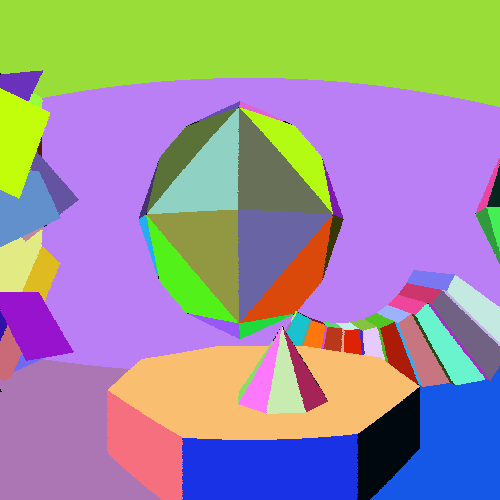
\includegraphics[width=\textwidth]{images/synthetic_ds.png}
        \caption[3D-KHT Accumulator Array]{}
        \label{fig:synth}
    \end{subfigure}
    \hspace{\fill}
    \begin{subfigure}{0.45\textwidth}
        \centering
        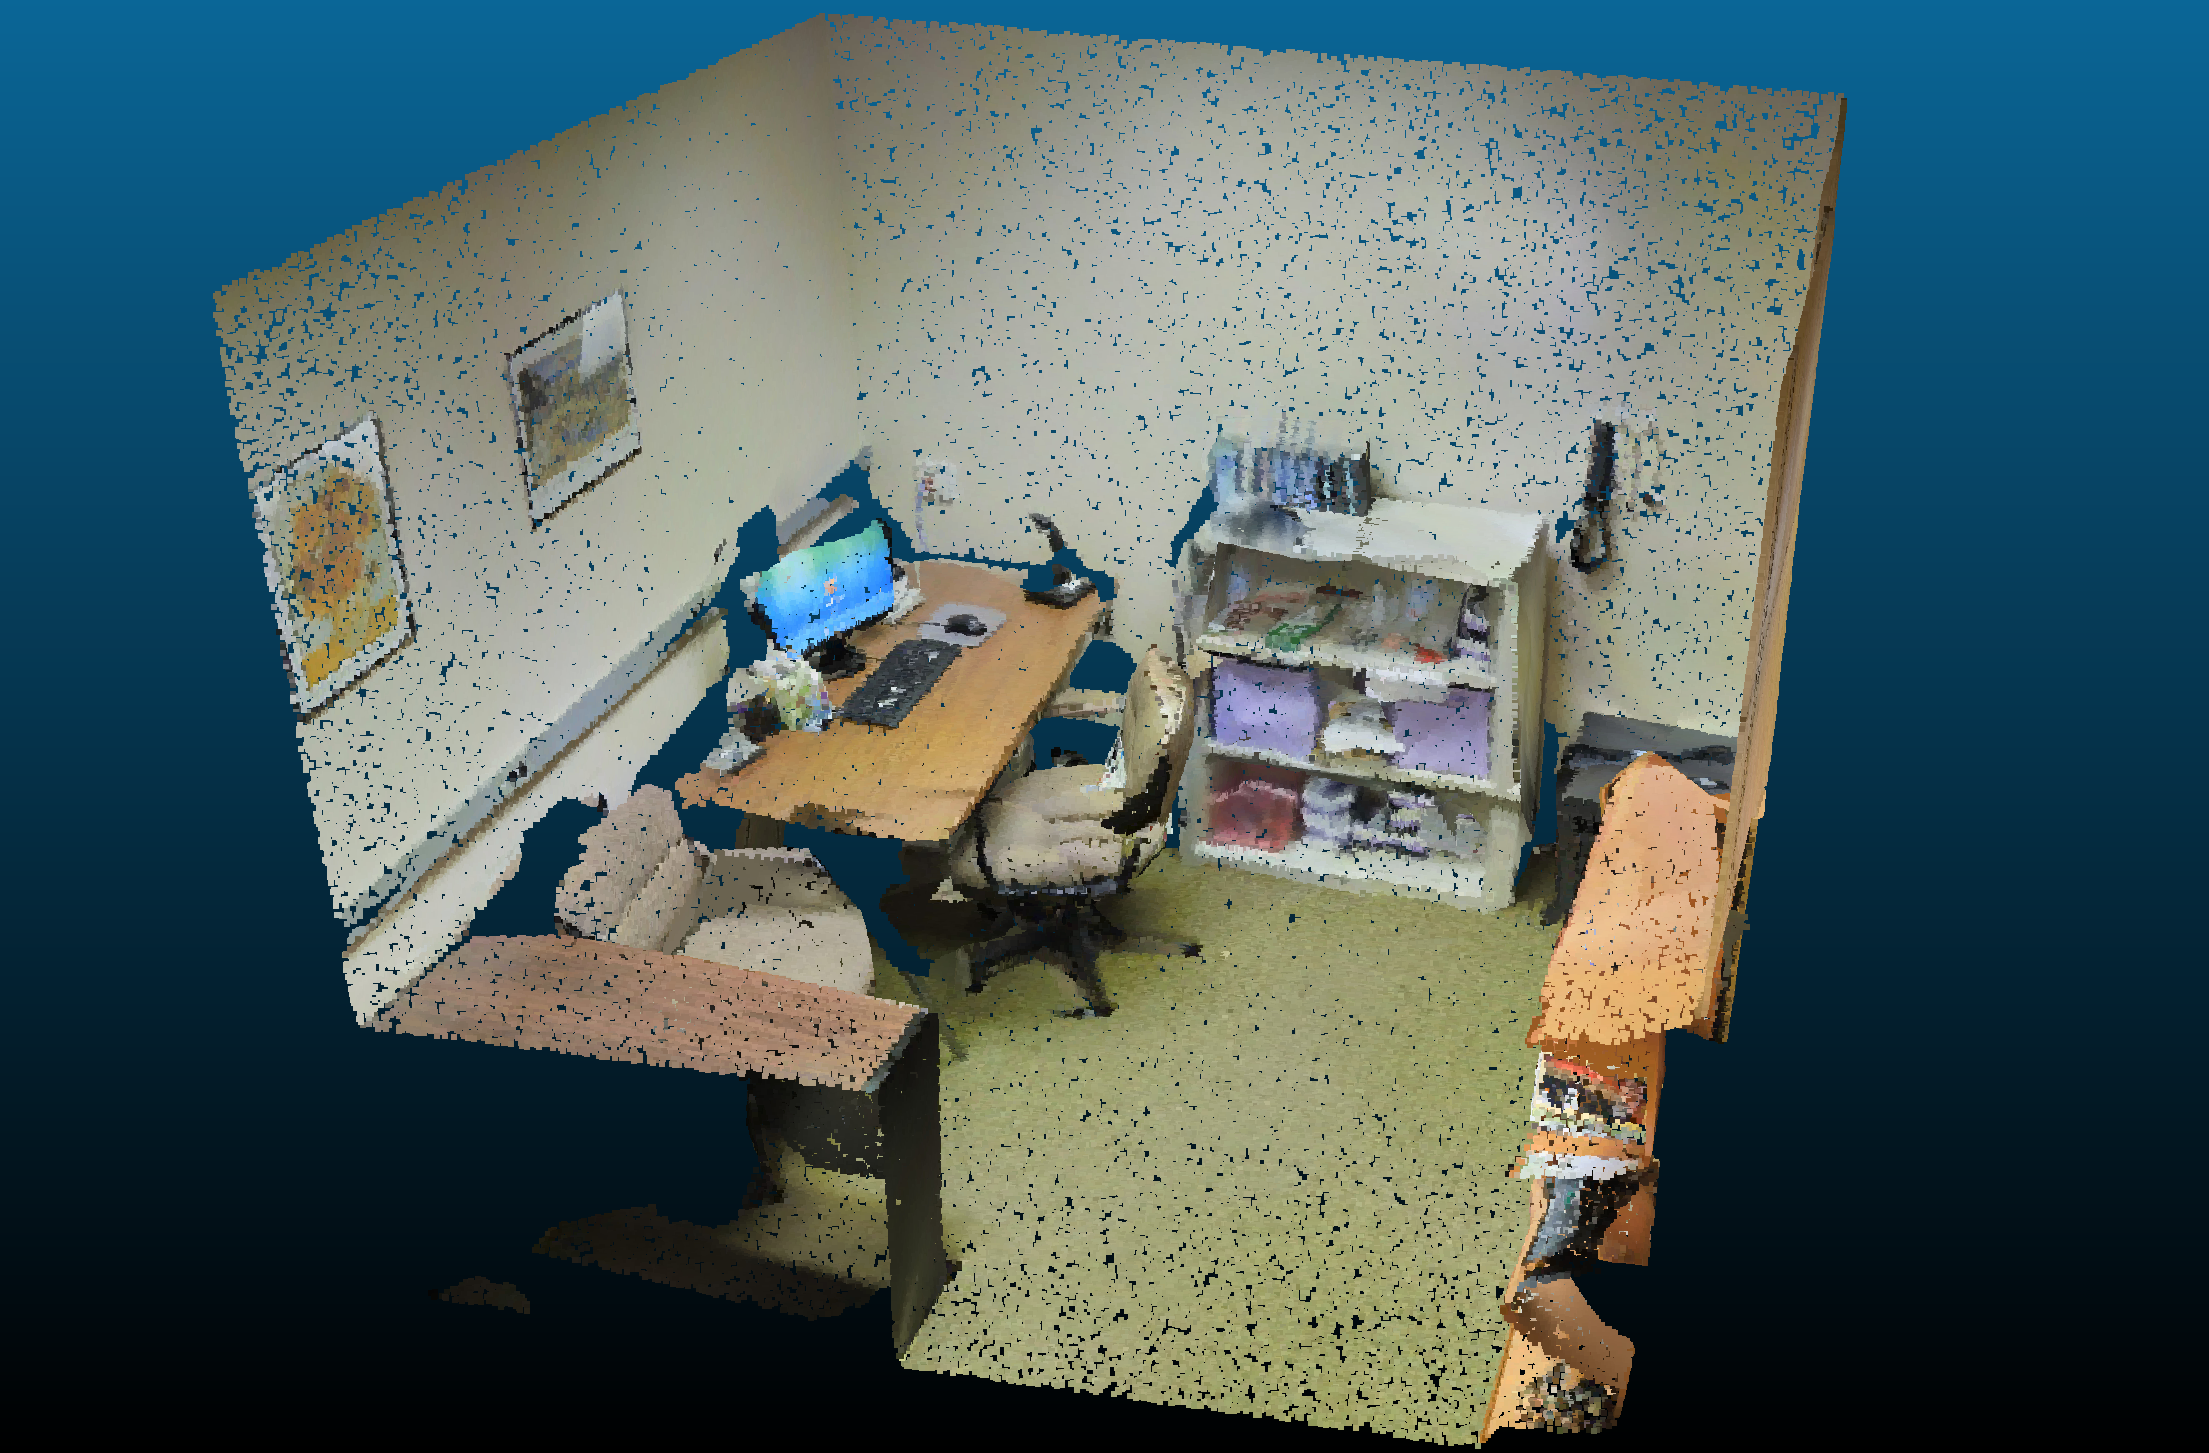
\includegraphics[width=\textwidth]{images/real_ds.png}
        \caption[3D-KHT Accumulator Ball]{}
        \label{fig:real}
    \end{subfigure}
    \hspace{\fill}
    \caption[Synthetic and Realistic Dataset Comparison]{A synthetic dataset (a) and a real office scene (b).
        The former is from the \textit{SegComp}~\cite{article} dataset, and the latter is from the \textit{2D-3D-S}~\cite{2017arXiv170201105A} dataset.
        Note that we cropped the office point cloud for visualization purposes.}
    \label{fig:ds_realism}
\end{figure}


\paragraph{Recorded Environment}
Since \textit{realistic} datasets are created through manual recording, it is useful to
differentiate between \textit{indoor} and \textit{outdoor} environments.
Note that we consider this criterion only to apply for \textit{real} datasets as \textit{synthetic}
datasets are not recorded manually.

\paragraph{Ground Truth}
Lastly, not all datasets are created out of the same motivation. Therefore, the method of evaluation differs widely over the range of available datasets.
In general, the \textit{Ground Truth} (GT) of currently popular datasets can fall into one of the following categories:

\begin{itemize}
    \item Planes,
    \item classes, \textit{or}
    \item trajectory.
\end{itemize}

A \textit{Ground Truth} can represent the detectable planes in a scene.
Therein, the format of the planes depends on the \textit{Plane Format} of the algorithm (see Paragraph~\ref{subsec:planeformat}).

Often, datasets from the field of semantic segmenation or object detection are used for the evaluation of plane detection algorithms.
Therein, all, or most, objects of a scene are assigned specific \textit{object classes}, e.g., "Wall", "Ceiling", "Table", or "Cup".
The \textit{Ground Truth} provides a labeling of these objects. This labeling can take the form of annotated 3D bounding boxes or sets of
pixels in the input image.

Lastly, some datasets provide a $GT$ that focuses on the trajectory of the recording sensor.

Naturally, this classification can only apply to datasets that include a \textit{Grund Truth}

\subsection{Datasets}
Table~\ref{tab:datasets} summarizes datasets currently prevalent in the scientific literature regarding plane detection.
Most of the datasets therein are used in the corresponding papers of the plane detection algorithms presented in Table~\ref{tab:algos}.
However, this does not influence the selection process. The table shows the respective classifications of each algorithm according to the criteria above.
Note that \textit{SYNPEB} and \textit{SegComp} are \textit{synthetic} datasets and, therefore, are neither \textit{indoor} nor \textit{outdoor}.
Furthermore, we are not aware of a \textit{ground truth} for the \textit{ARCO} dataset.

\begin{table}[H]
    \centering
    \caption[Popular Datasets]{Plane detection Datasets. The \textit{GT}(Ground Truth) column specifies what the ground truth of each dataset represents.
        The datasets are clustered by their type of format. The remaining order is arbitrary.
        The second column "Section" provides the placement within this work.
        Note that we include our dataset (FIN) in this table for completeness reasons.
    }

    \resizebox{\textwidth}{!}{%
        \begin{tabular}{cccccc}
            \toprule
            \textbf{Dataset}                                                                                                                                                                      & \textbf{Section}         & \textbf{Scene Format} & \textbf{Real} & \textbf{Indoor} & \textbf{GT} \\
            \midrule
            \textbf{2D-3D-S}      \cite{2017arXiv170201105A}                                                                                                                                      & \ref{subsec:bg-stanford} & UPC                   & Y             & Y               & classes     \\
            \textbf{Leica\tablefootnote{\href{https://shop.leica-geosystems.com/de/leica-blk/blk360/dataset-downloads}{https://shop.leica-geosystems.com/de/leica-blk/blk360/dataset-downloads}}} & \ref{subsec:bg-Leica}    & UPC                   & Y             & N               & planes      \\
            \textbf{Kinect}      \cite{Oehler_Stueckler_Welle_Schulz_Behnke_2011}                                                                                                                 & \ref{subsec:bg-Kinect}   & OPC                   & Y             & Y               & planes      \\
            \textbf{SYNPEB}      \cite{schaefer19icra}                                                                                                                                            & \ref{subsec:bg-SYNPEB}   & OPC                   & N             & /               & planes      \\
            \textbf{ARCO}        \cite{Hidalgo-Paniagua_Vega-Rodriguez_Pavón_Ferruz_2015}                                                                                                         & \ref{subsec:bg-ARCO}     & OPC                   & Y             & Y               & /           \\
            \textbf{SegComp}     \cite{article}                                                                                                                                                   & \ref{subsec:bg-segcomp}  & DI                    & N             & /               & planes      \\
            \textbf{NYU V2}      \cite{10.1007/978-3-642-33715-4_54}                                                                                                                              & \ref{subsec:bg-NYU}      & DI                    & Y             & Y               & classes     \\
            \textbf{ICL-NUIM}    \cite{handa:etal:ICRA2014}                                                                                                                                       & \ref{subsec:bg-ICL}      & DI                    & Y             & Y               & trajectory  \\
            \textbf{SUNRGB-D}         \cite{7298655}                                                                                                                                              & \ref{subsec:bg-SUN}      & DI                    & Y             & Y               & classes     \\
            \textbf{TUM}         \cite{sturm12iros}                                                                                                                                               & \ref{subsec:bg-TUM}      & DI                    & Y             & Y               & trajectory  \\
            \midrule
            \textbf{FIN (ours)}                                                                                                                                                                   & \ref{sec:finimpl}        & UPC                   & Y             & Y               & planes      \\
            \bottomrule
        \end{tabular}
    }
    \label{tab:datasets}
\end{table}


In Subsection~\ref{subsec:pdaselect}, we determine \textit{unorganized} point clouds as the type of input.
Furthermore, since we give special focus to the real-world applicability of plane detection algorithms, we must evaluate them on \textit{realistic} datasets, thereby excluding all datasets except \textit{2D-3D-S} and \textit{Leica}. 
Lastly, we are especially interested in realistic \textit{indoor} environments, as motivated by Chapter~\ref{chap:Introduction}.
Therefore, \textit{Leica} ceases to be an option and we subsequently choose \textit{2D-3D-S} as the dataset for the evaluation.


Nevertheless, we cannot use the ground truth included in \textit{2D-3D-S} because it represents the segmented scene at the level of objects instead of focusing on layers within the scene.
As a consequence thereof, we create a suitable ground truth of the \textit{2D-3D-S} dataset through manual segmentation.
We provide details of this time-expensive process in Section~\ref{sec:gtseg}.


Lastly, \textit{2D-3D-S} does not inherit any temporal component, i.e., the \textit{unorganized} point clouds do not grow incrementally over time.
To the best of our knowledge, there exists no dataset that meets the above criteria and, additionally, provides a plane-focused ground truth.
Therefore, we record an incrementally growing dataset in the Faculty of Computer Science at Otto-von-Guericke University Magdeburg,
henceforth referred to as the \textit{FIN} dataset.



To perform a thorough comparison between the \textit{FIN} and \textit{2D-3D-S}, and, subsequently, between the static and the dynamic dataset, we record a scene for each of the following scene types:
\begin{itemize}
    \item office
    \item conference room
    \item auditorium
    \item hallway
\end{itemize}

We focus on these four scene types because they are the most common in a realistic indoor environment.
The recorded point clouds can be seen in Figure~\ref{fig:fin}.
Lastly, since this is a novel dataset and thus has no ground truth, we create a ground truth. The details thereof are explained in Section~\ref{sec:finimpl}.


\begin{figure}[H]
    \begin{subfigure}{0.5\textwidth}
        \centering
        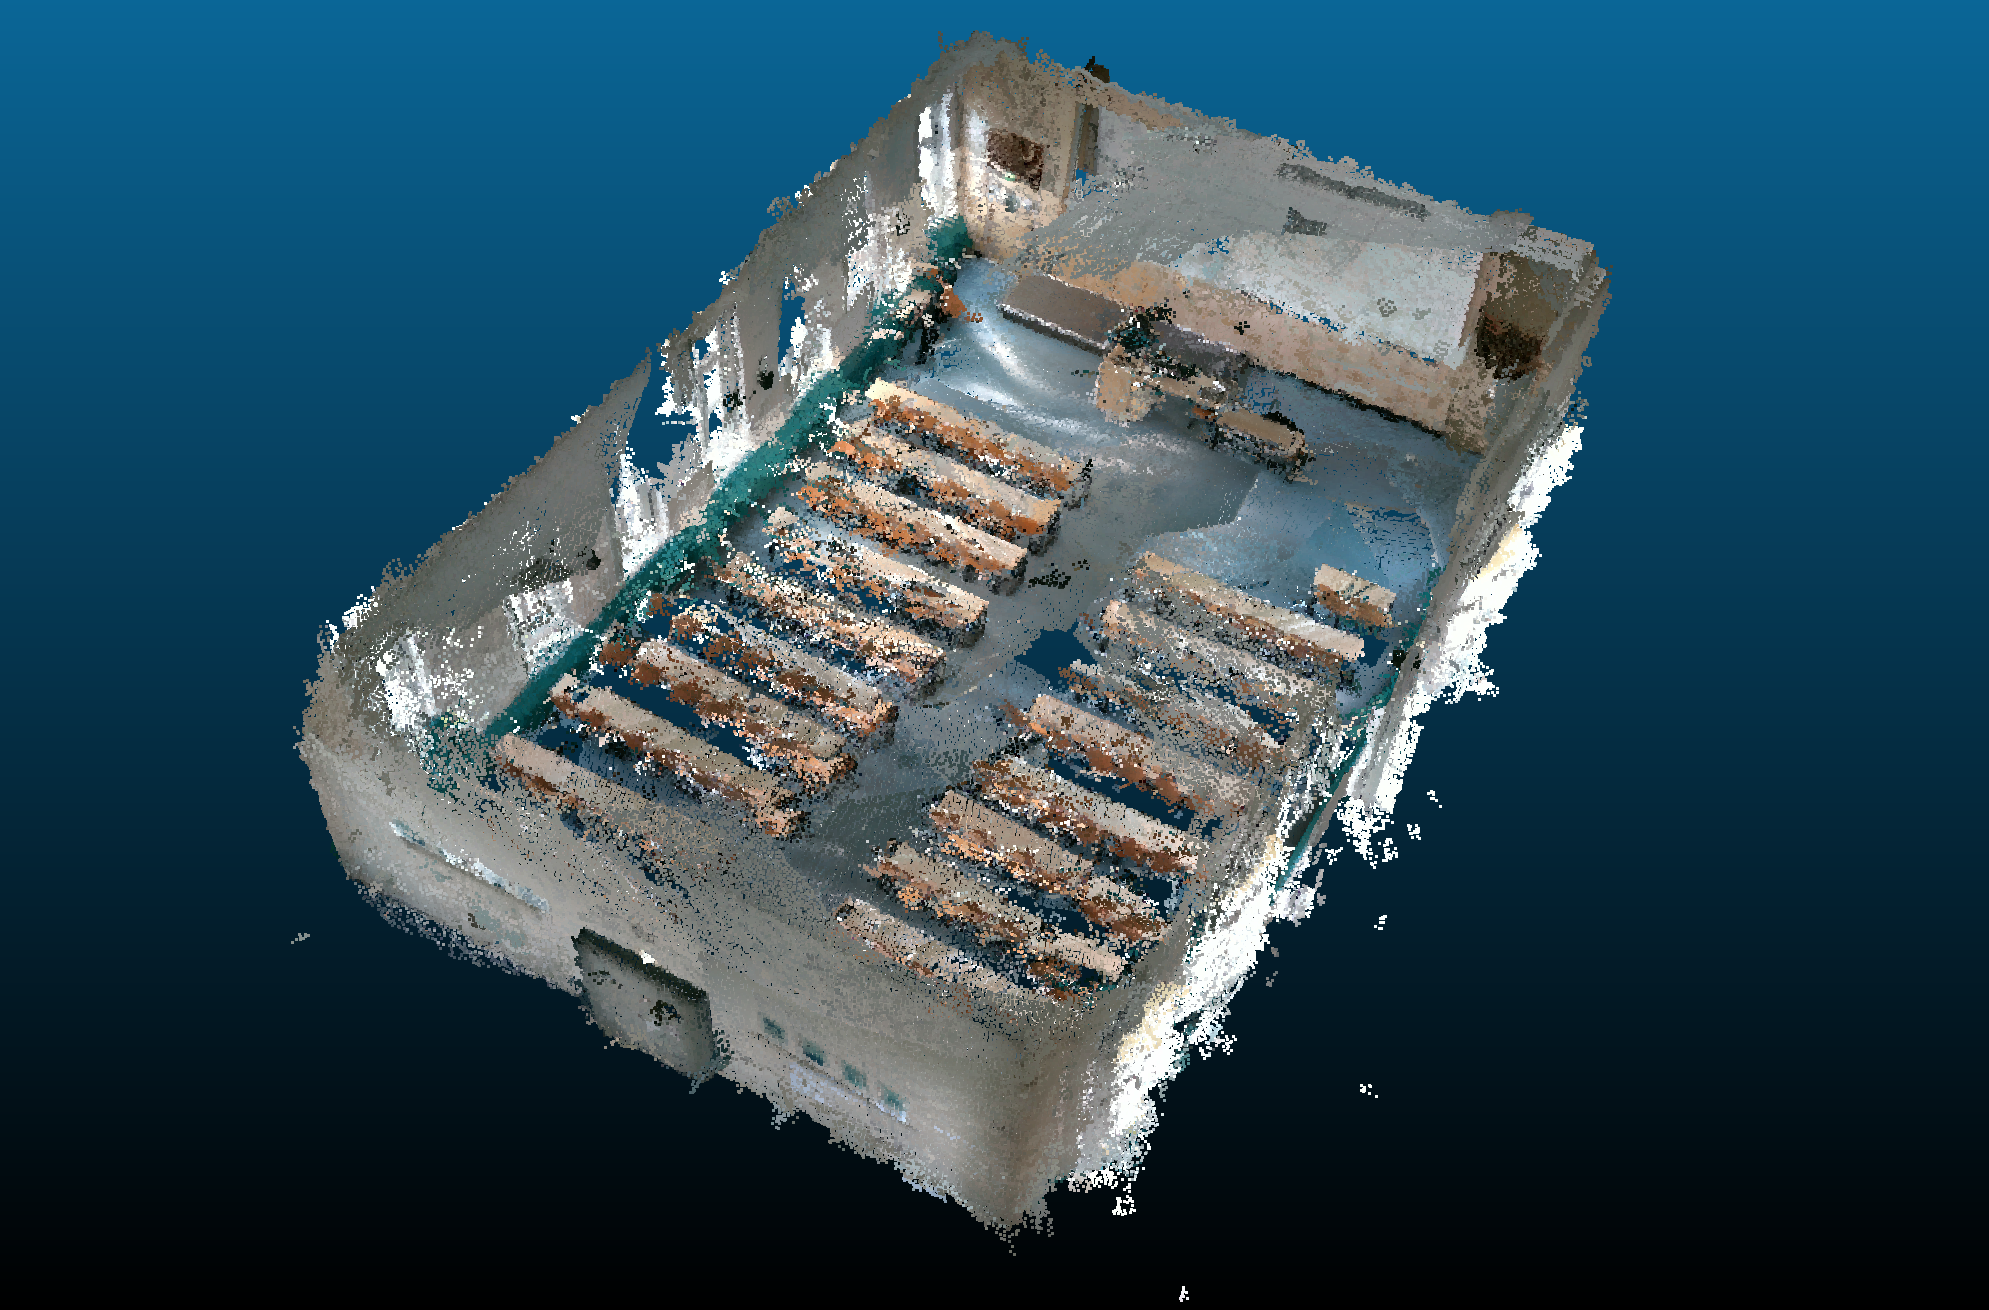
\includegraphics[width=.9\linewidth]{images/307.png}
        \caption[Dynamic Dataset - auditorium]{}
        \label{fig:fin307}
    \end{subfigure}
    \begin{subfigure}{0.5\textwidth}
        \centering
        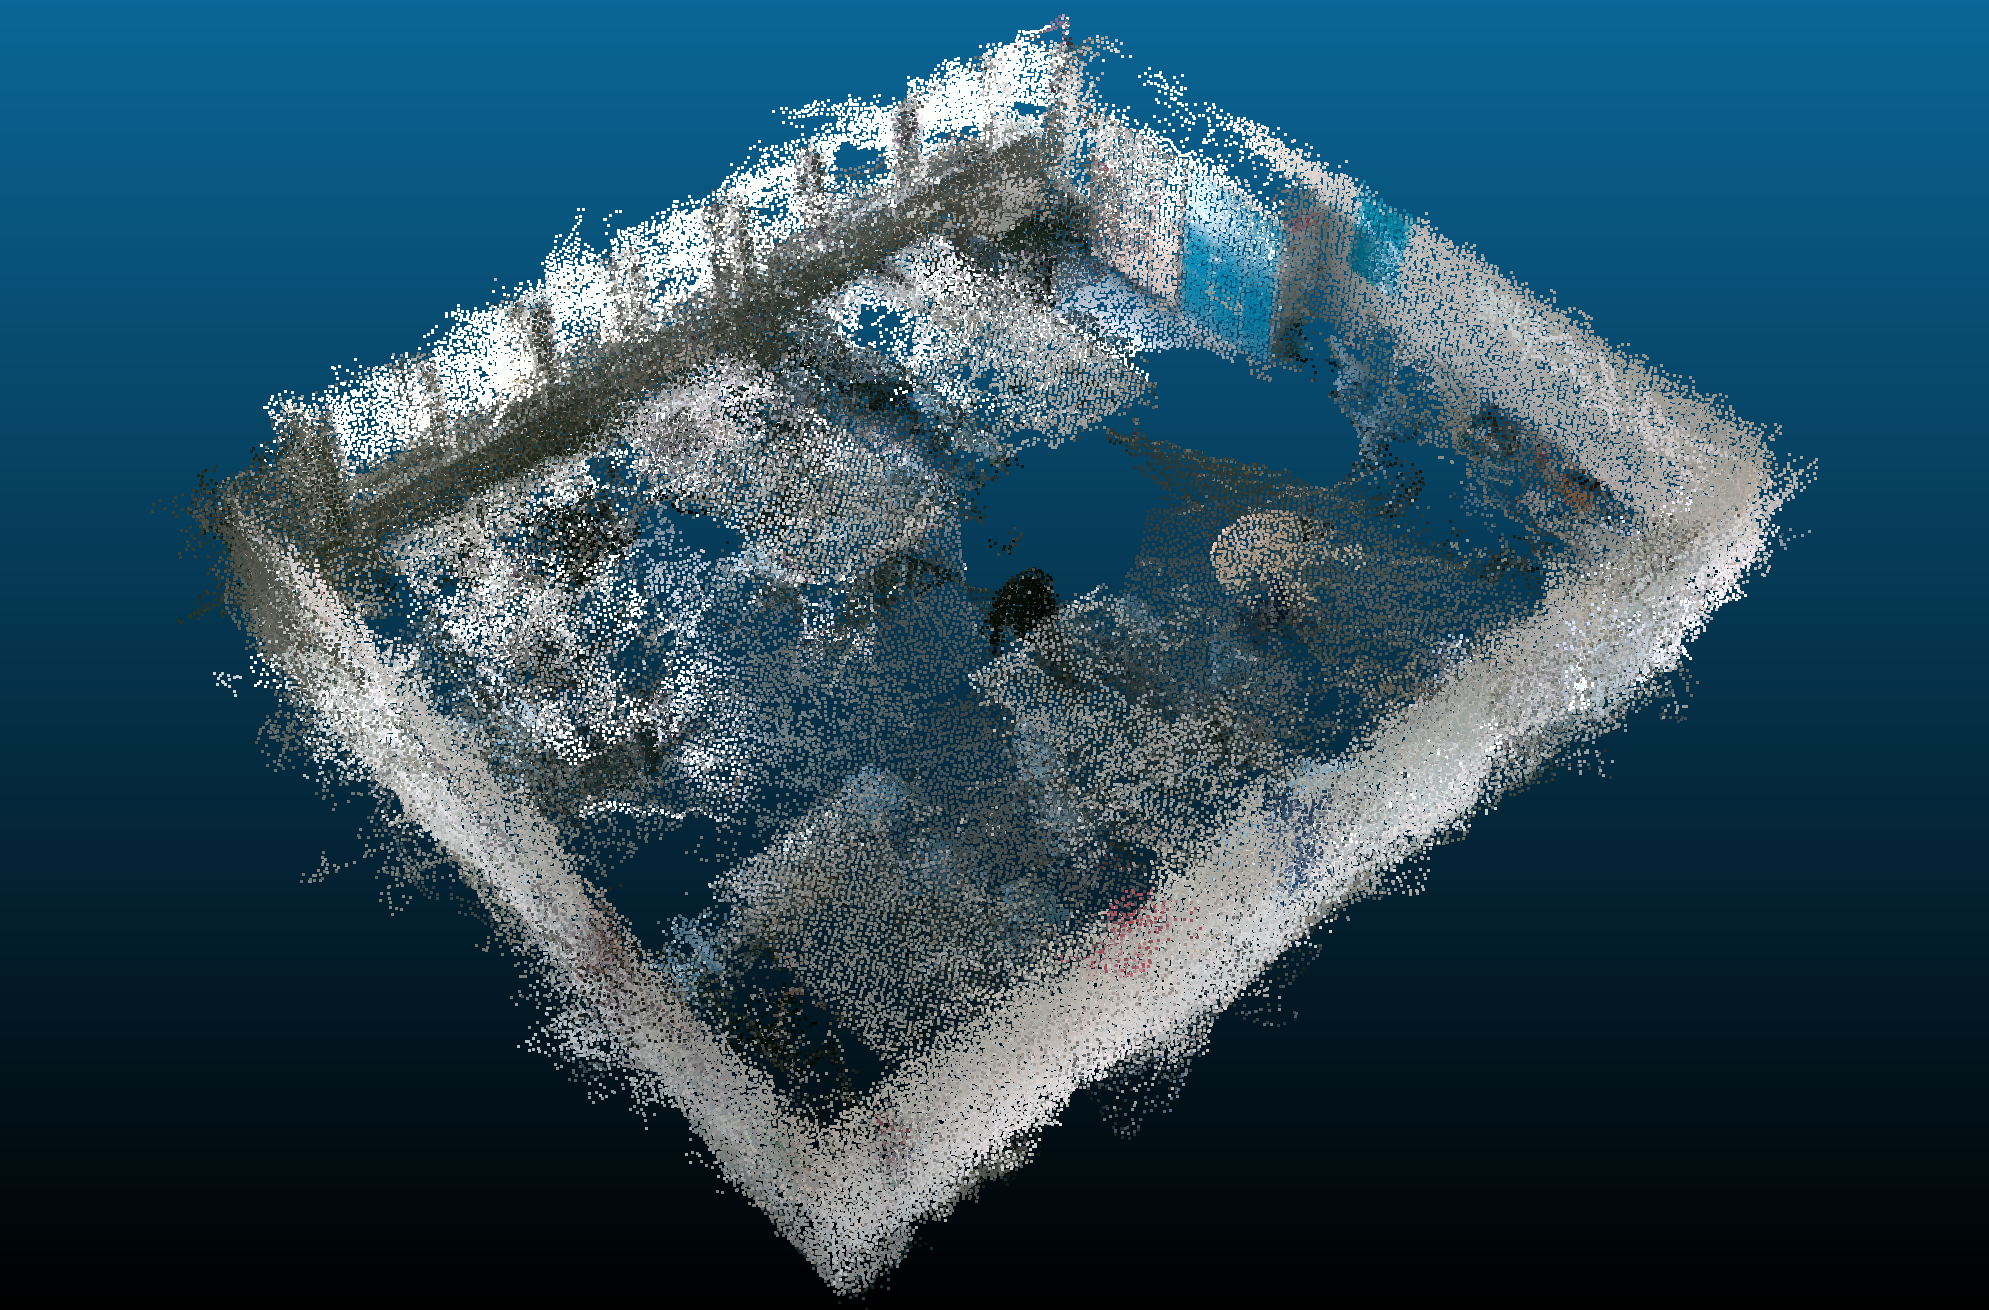
\includegraphics[width=.9\linewidth]{images/333.png}
        \caption[Dynamic Dataset - conference room]{}
        \label{fig:fin333}
    \end{subfigure}
    \begin{subfigure}{0.5\textwidth}
        \centering
        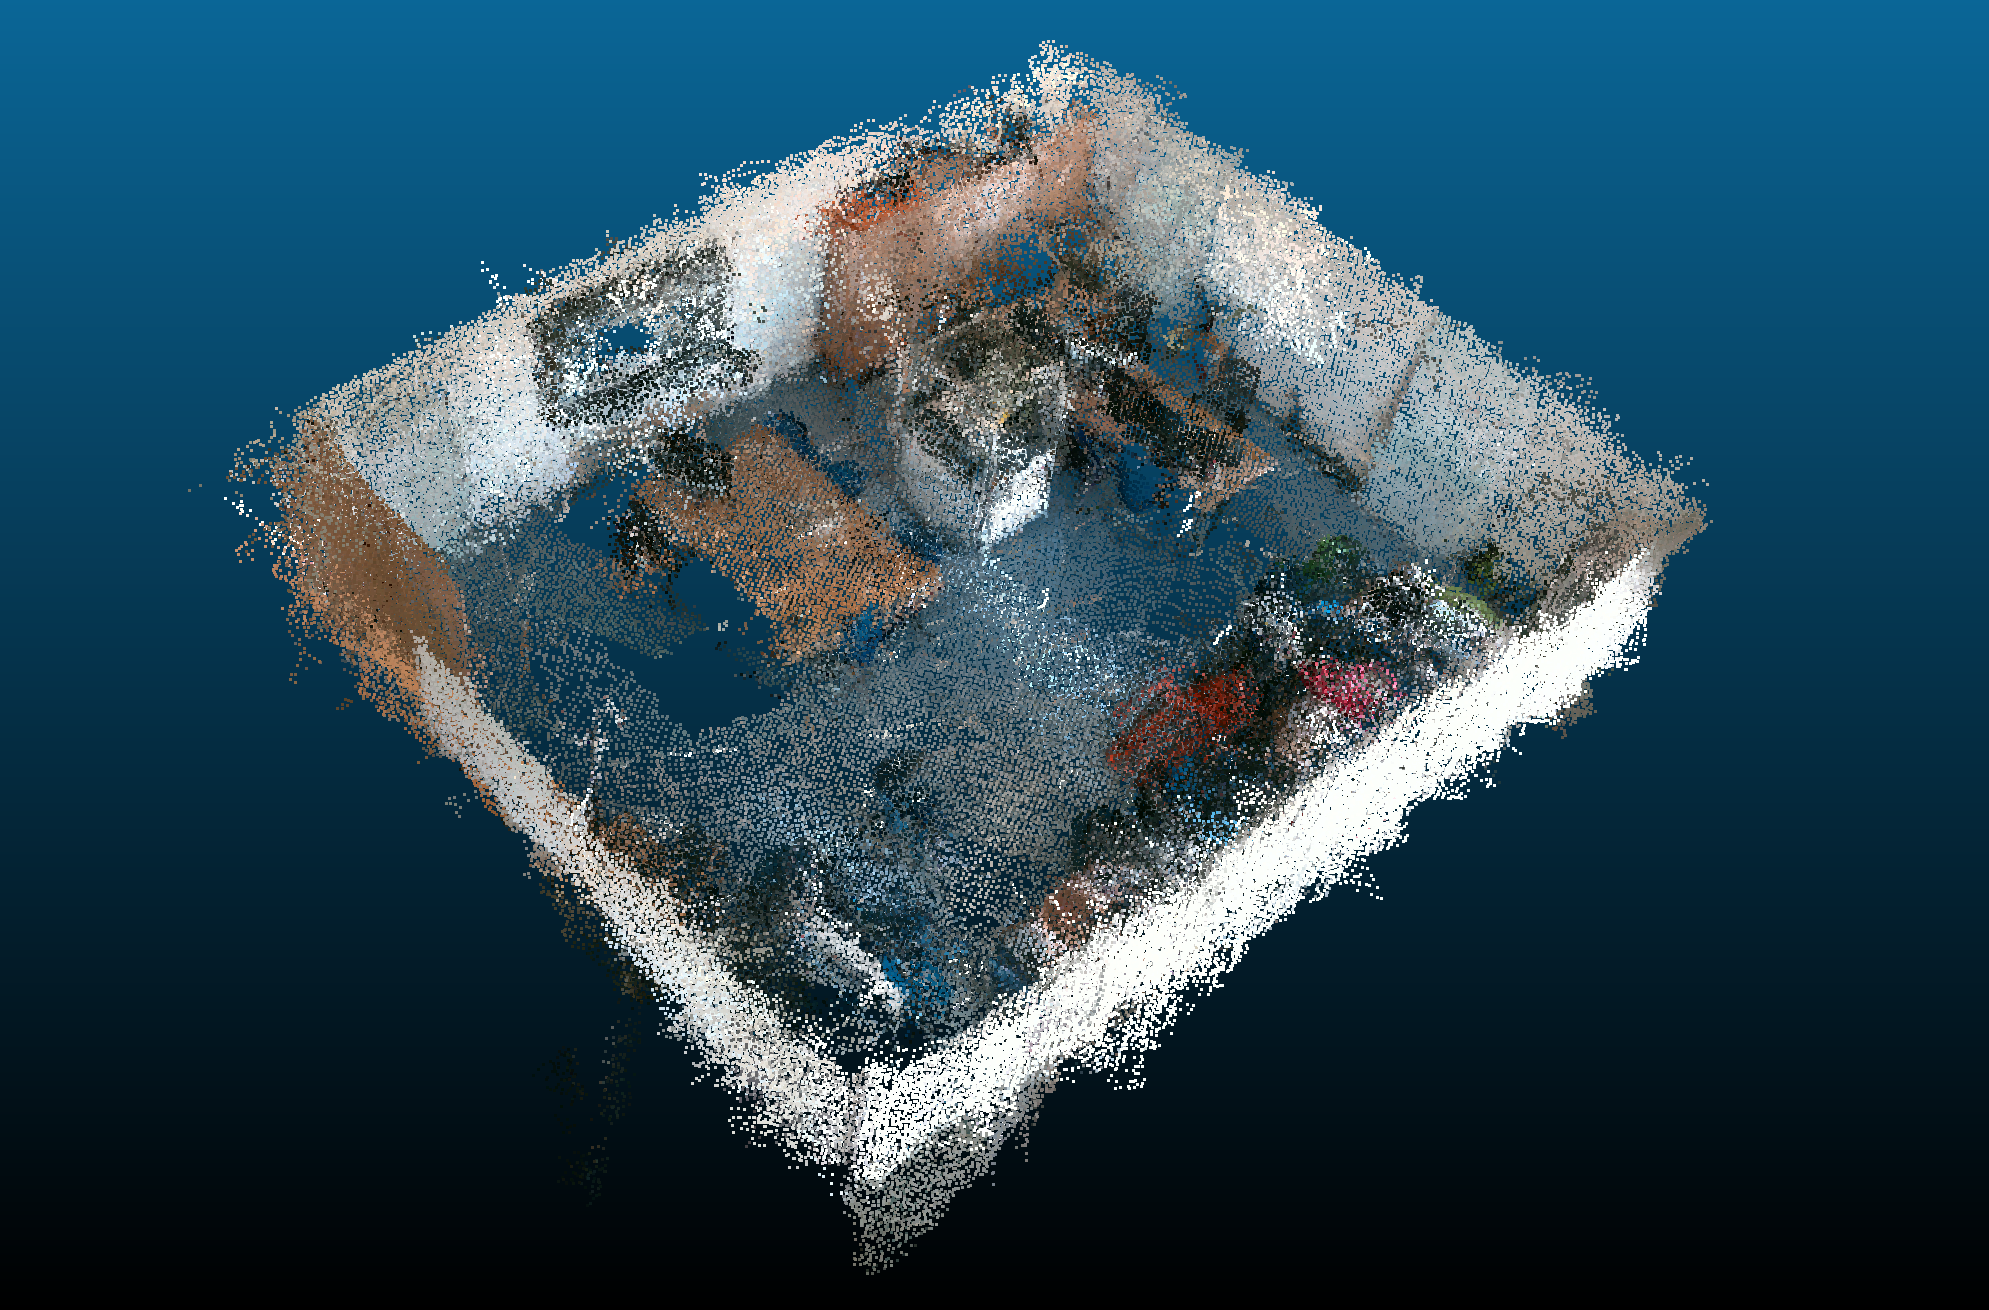
\includegraphics[width=0.9\linewidth]{images/425.png}
        \caption[Dynamic Dataset office]{}
        \label{fig:fin425}
    \end{subfigure}
    \begin{subfigure}{0.5\textwidth}
        \centering
        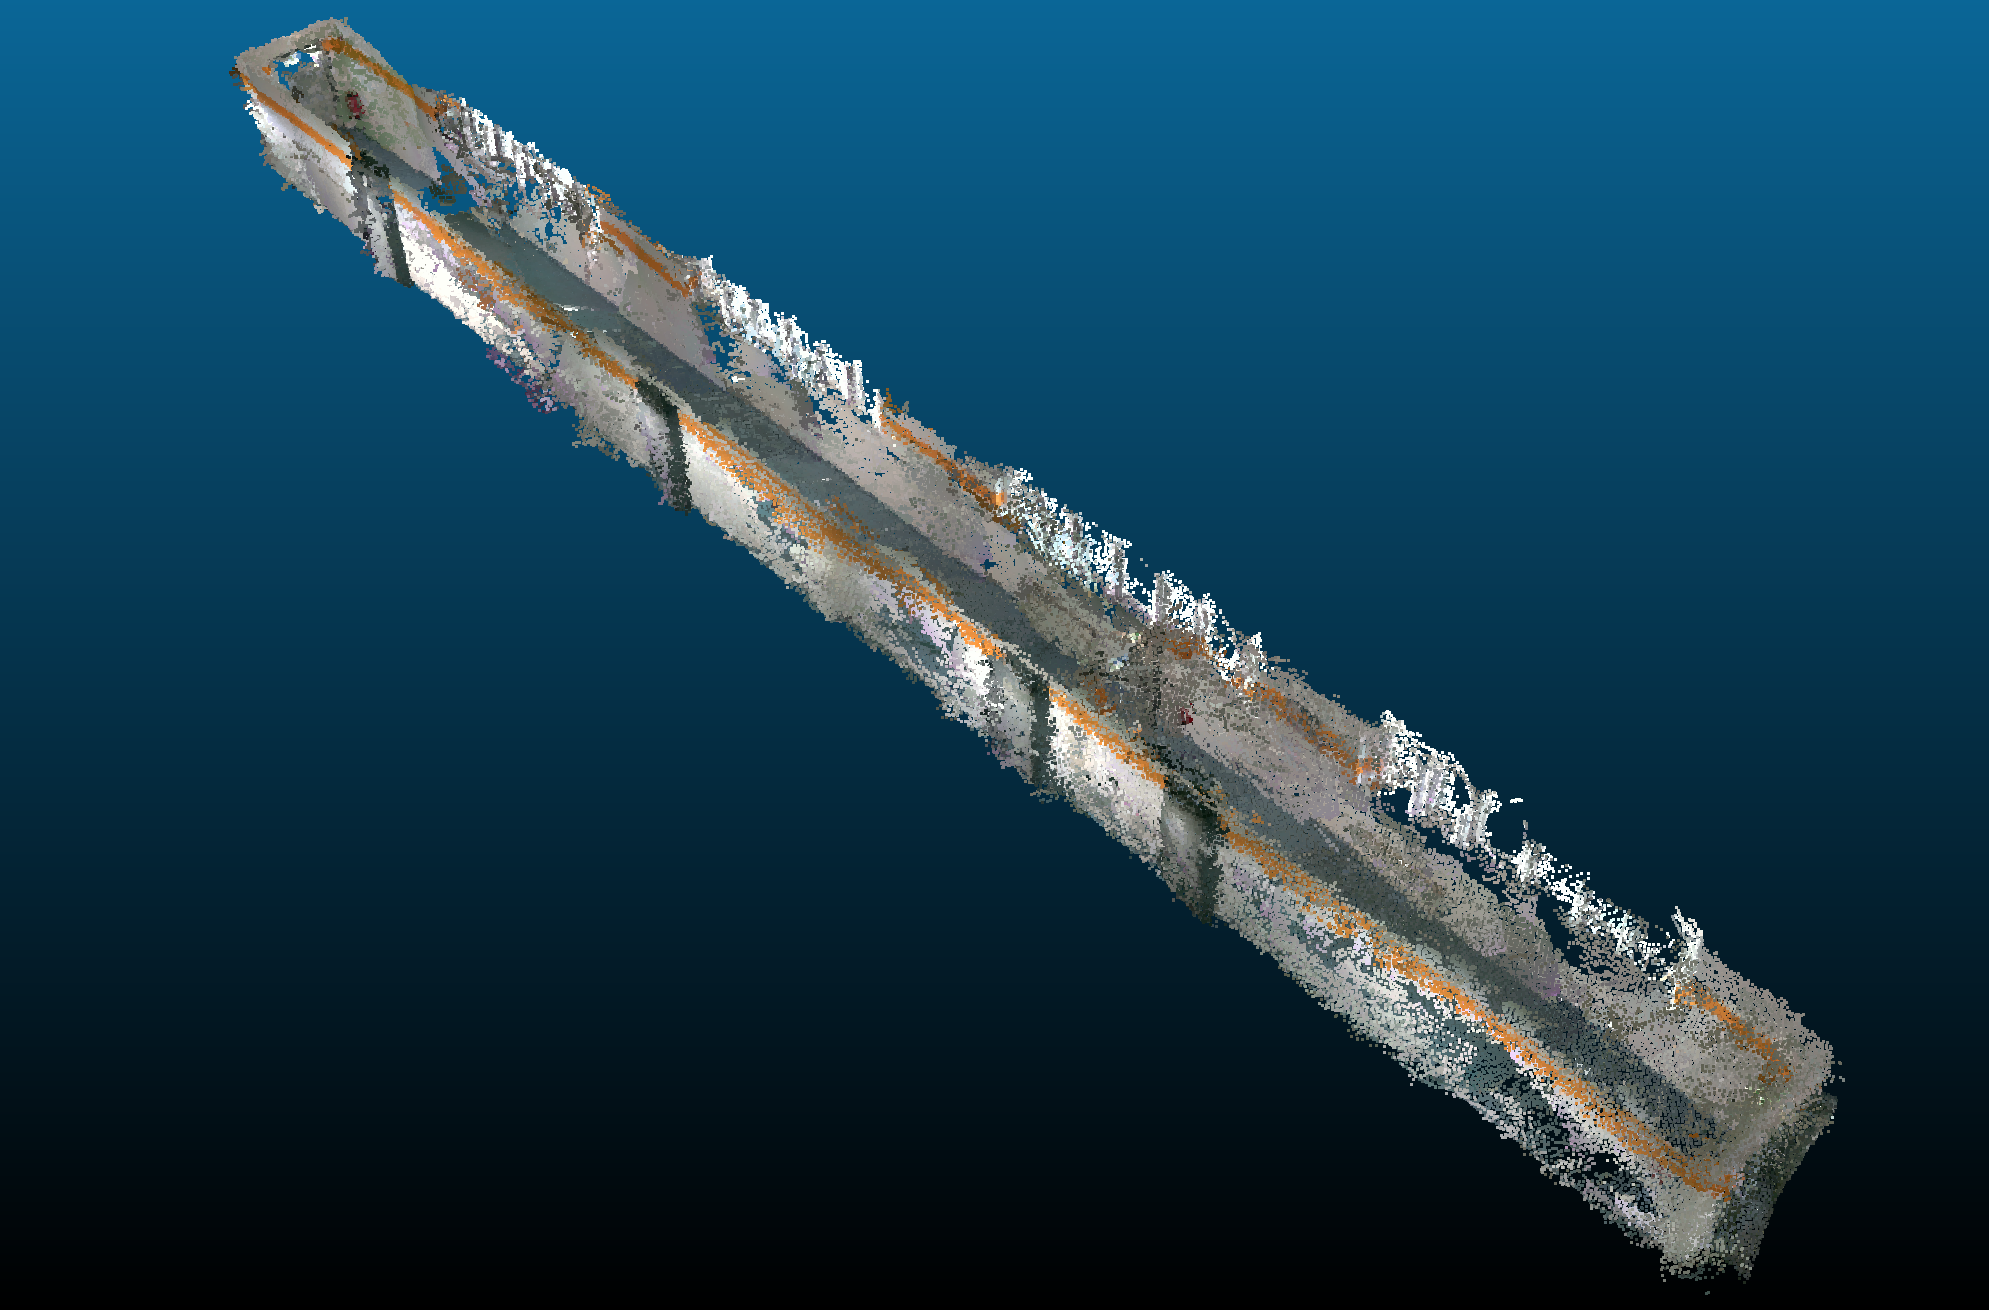
\includegraphics[width=0.9\linewidth]{images/hallway.png}
        \caption[Dynamic Dataset office]{}
        \label{fig:finhw}
    \end{subfigure}
    \caption[Dynamic Datasets]{The recorded point clouds for each scene type: (a) auditorium, (b) conference room, (c) office and (d) hallway.
        The ceilings have been manually removed for visualization purposes but remain in the dataset for the experiments.}
    \label{fig:fin}
\end{figure}


\section{Definition Real-Time}\label{sec:realtime}
Finally, as mentioned in the beginning of Chapter~\ref{chap:Concept}, we must define the meaning of real-time to determine the \textit{real-time} applicability of a plane detection algorithm.


In Subsection~\ref{subsec:pdaselect}, we introduce the differentiation between pre-processing and post-processing steps.
It is possible that one phase of an algorithm accounts for the majority of the total calculation time and that the algorithm
would be considered \textit{real-time} applicable, if that phase were to be excluded.
Because some steps can be covered by previous steps in the AR/VR system (see Figure~\ref{fig:concept}), i.e., by the sensor or the SLAM algorithm,
we give two definitions of \textit{real-time}.

In general, and without taking the algorithms internal structure into consideration, we have to consider possible
hardware limitations, data flow, and how often it is needed to perform calculations, e.g., how quickly the SLAM algorithm
updates its internal map (Figure~\ref{fig:concept}, [2]) or how frequently new planes are needed (Figure~\ref{fig:concept}, [4]).
The recorded raw data is not directly sent to the plane detection algorithm but instead given to RTAB-MAP, which then performs
calculations to update and publish the map.
Therefore, the upper limit is the frequency of how often RTAB-MAP publishes those updates, which by default is once per second.

\paragraph{Total Real-Time $\mathbf{RT_{tot}}$}
According to this upper limit of RTAB-MAP, we consider an algorithm \textit{totally Real-Time} applicable, if it achieves an average frame
rate of minimum 1, e.g., the total processing time of an algorithm lies under one second. In the remainder of this work, we
use \textit{total Real-Time} and $RT_{tot}$ interchangeably.

\paragraph{Real-Time Plane Calculation $\mathbf{RT_{calc}}$}
Being a subset of \textit{totally Real-Time applicability, Real-Time Plane Calculation} determines the real-time applicability if the processing time of an algorithm
\textit{excluding} pre-processing lies under the aforementioned upper bound of $1s$. Like $RT_{tot}$, we use
\textit{Real-Time Plane Calculation} and $RT_{calc}$ interchangeably.

%TODO  Eig nur needed wenn die algos langsamer sind als 1s ODER sollte die cloud extrem wachsen kann man sich auf die 6 meter beschränken, erstmal aber nicht}\\
% \subsection*{reduktion (opt)}
% We can reduce complexity further by taking the specifications (background)
% of the D455 into account. The RMS error of the D455 is reported to be 2\% at 4 meters distance to the sensor.
% Furthermore, the ideal distance is stated to range between $0.6 - 6$ meters.
% To maintain a dense and precise representation of our environment, we therefore limit the detection of planes to a
% radius of 6 meters from the current position.

\section{Summary}
Many applications have constraints in the form of a temporal component. Augmented or Virtual Reality applications that include plane detection
are no exception. In addition to time constraints, good quality is often tightly coupled to expensive or closed technology.
In this work, we aim to evaluate the quality of real-time plane detection algorithms under the use of more affordable hardware, namely two Intel RealSense sensors. Therein, we are especially interested in the aspect of \textit{real-time} applicability in a realistic environment.

At the beginning of this chapter, we state that three aspects are required for this evaluation: A set of plane detection algorithms, useful datasets, and a definition
of real-time.
The selection of the best plane detection algorithm, however, is non-trivial. After defining meaningful criteria for objective judgement, we
select appropriate plane detection algorithms. Moreover, we select realistic datasets, one of which is a novel creation, and present two definitions of \textit{real-time} namely $RT_{tot}$ and $RT_{calc}$.
\end{document}